\chapter{Problema 1.1}

\section{Multiplexer 16:1}

Si chiede di progettare un multiplexer indirizzabile 16:1, utilizzando un approccio per composizione, utilizzando multiplexer 4:1.\\
Tale multiplexer è rappresentato di seguito.
\begin{figure}[H]
	\centering
	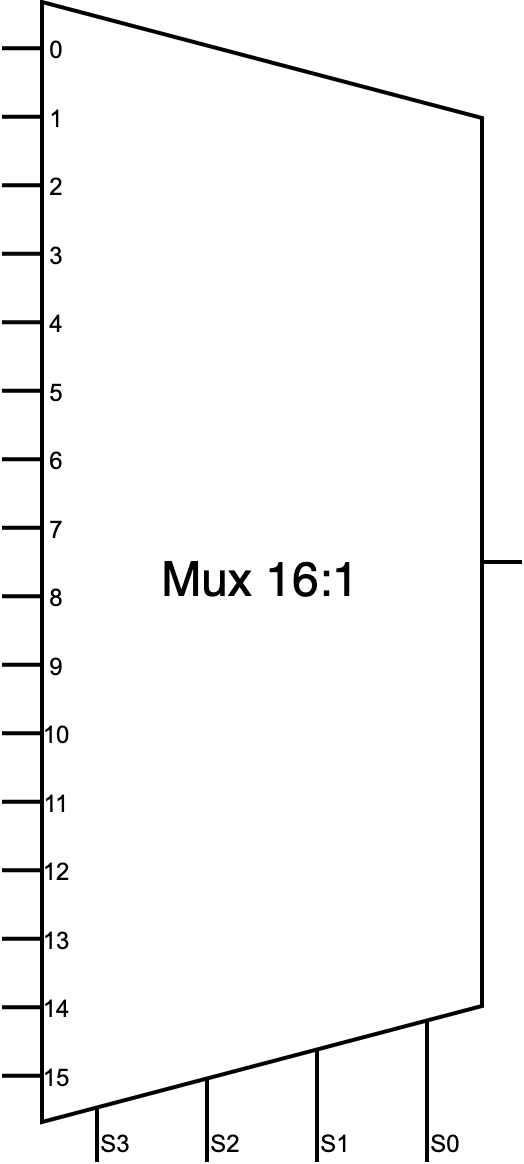
\includegraphics[width=0.3\textwidth]{img/01}
	\caption{multiplexer 16:1}
	\label{mux_16:1} 
\end{figure}

\subsection{Progetto e architettura}
Dapprima si utilizza un approccio per composizione per realizzare un multiplexer 4:1 con multiplexer 2:1.\\
\begin{figure}[H]
	\centering
	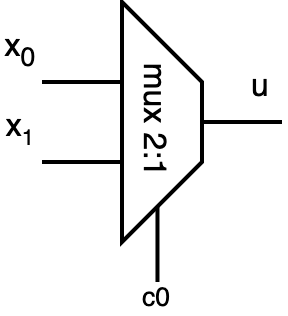
\includegraphics[width=0.3\textwidth]{img/02}
	\caption{multiplexer 2:1}
	\label{mux_2:1} 
\end{figure}
\begin{figure}[H]
	\centering
	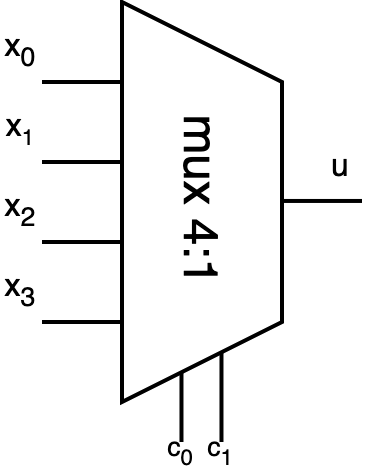
\includegraphics[width=0.2\textwidth]{img/03}
	\caption{multiplexer 4:1}
	\label{mux_4:1} 
\end{figure}
Si costruisce il multiplexer 4:1 come segue
\begin{figure}[H]
	\centering
	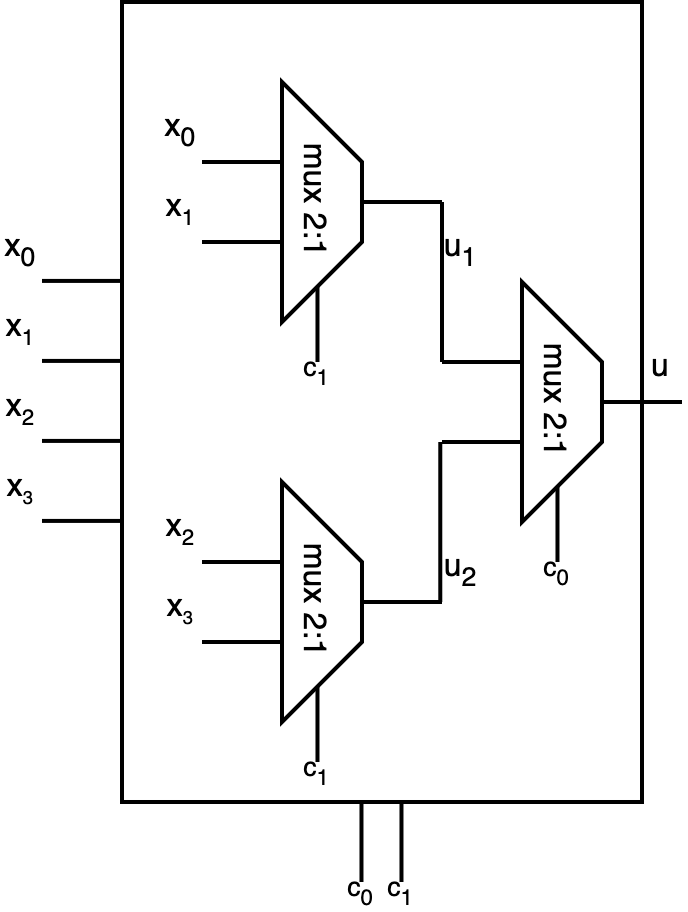
\includegraphics[width=0.4\textwidth]{img/04}
	\caption{multiplexer 4:1 per composizione di multiplexer 2:1}
	\label{mux_4:1_comp} 
\end{figure}
In maniera analoga si procede con la progettazione del multiplexer 16:1.
\begin{figure}[H]
	\centering
	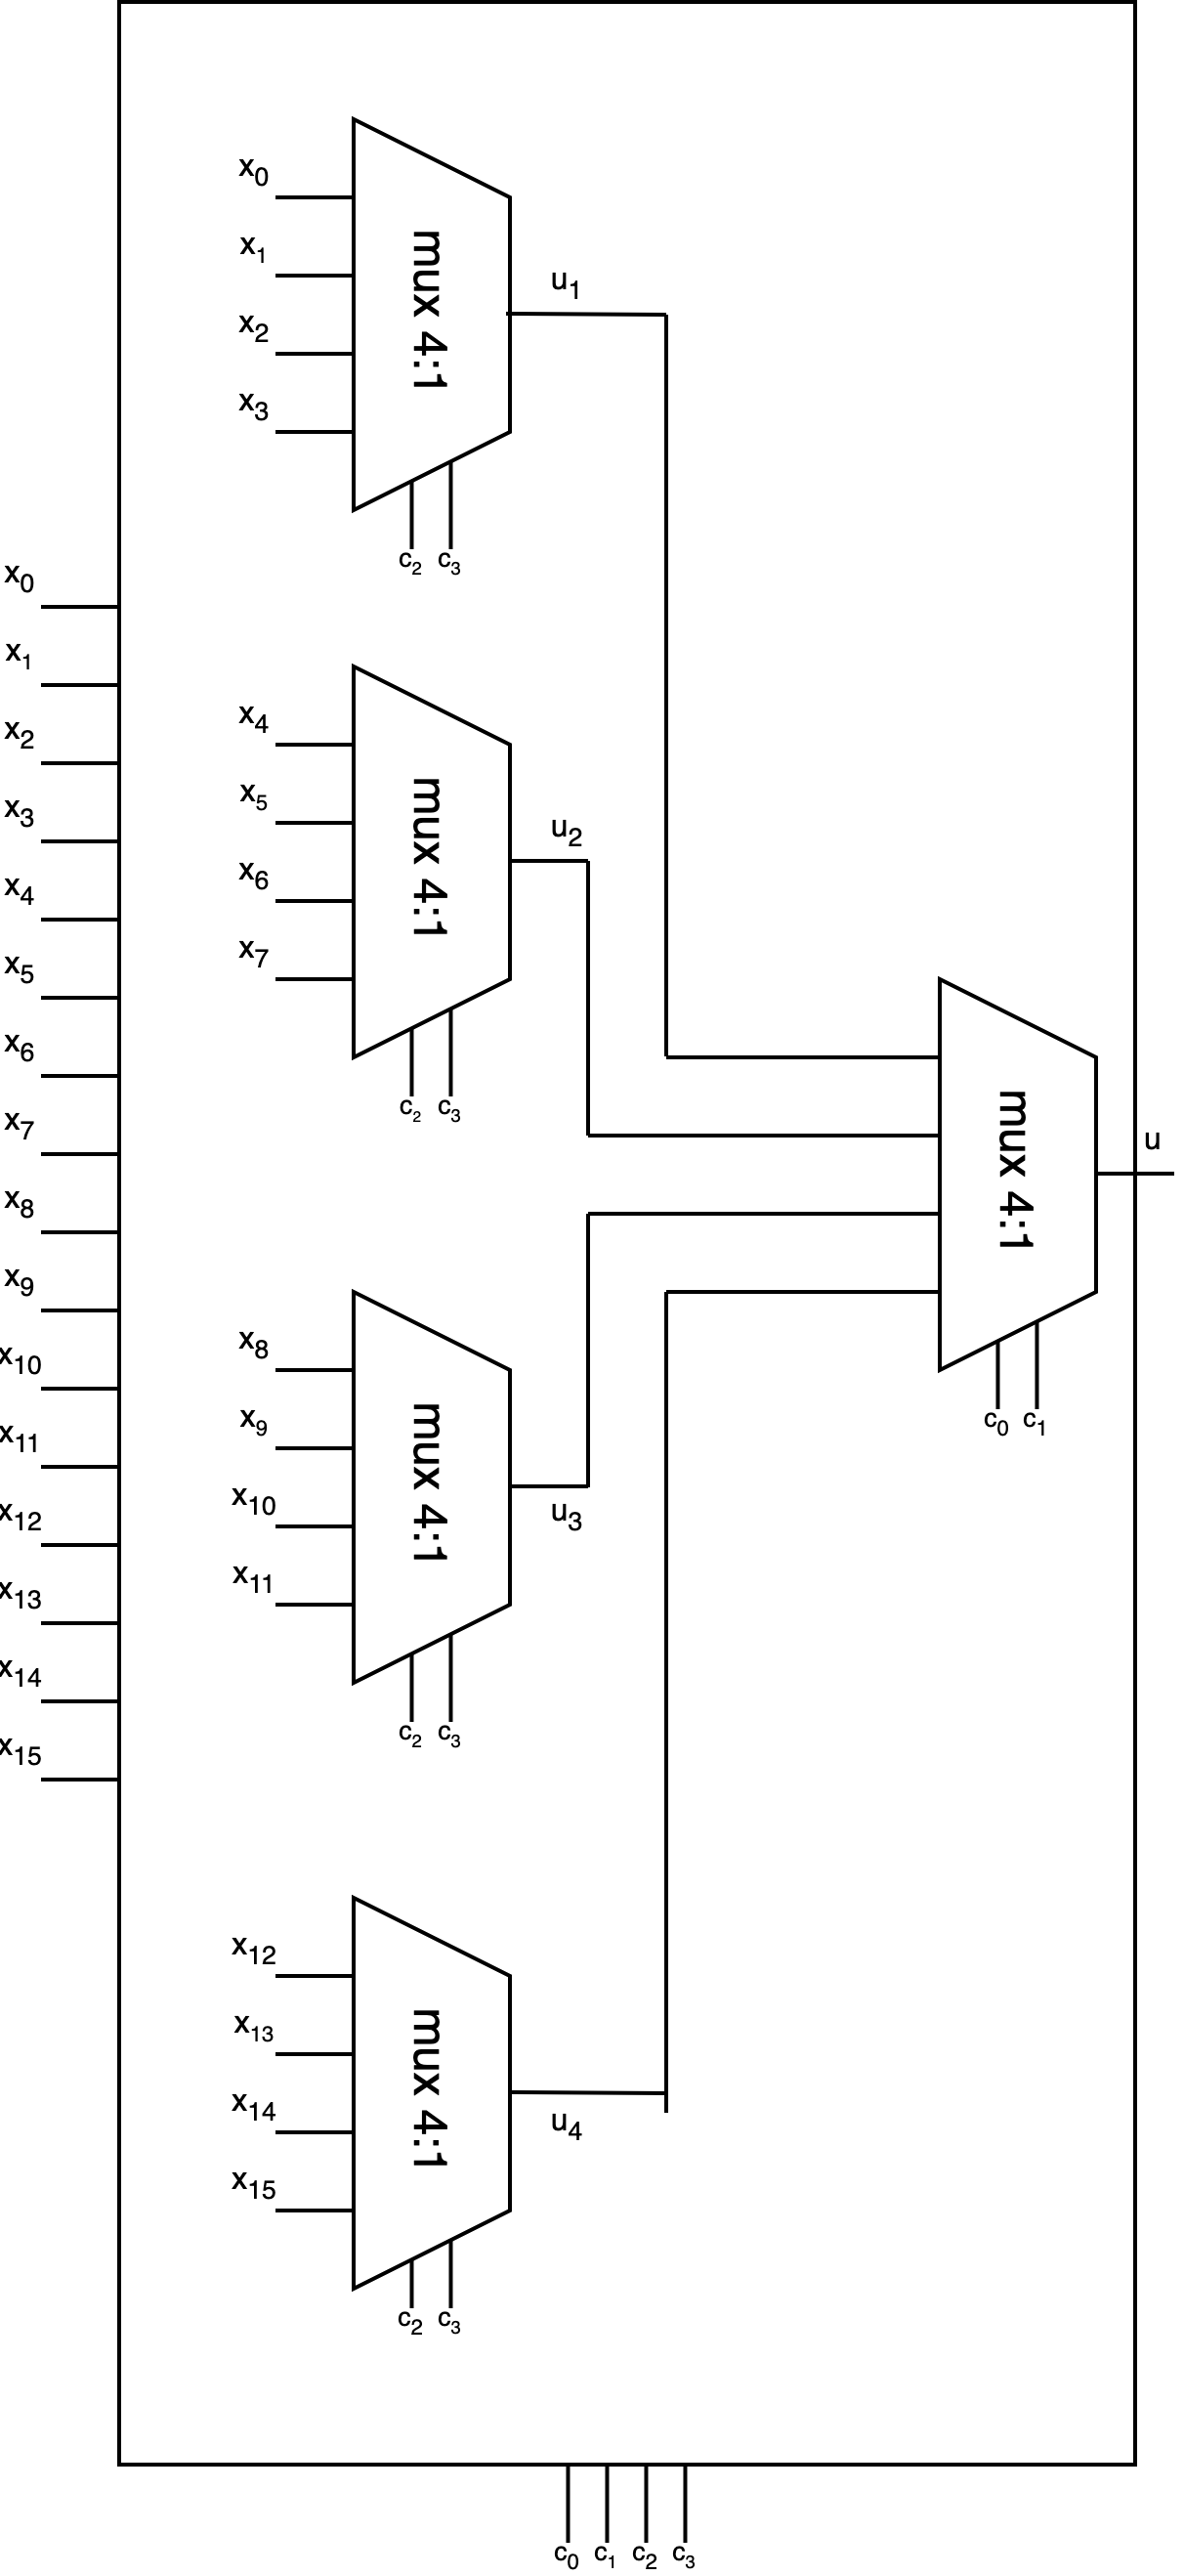
\includegraphics[width=0.4\textwidth]{img/05}
	\caption{multiplexer 16:1 per composizione di multiplexer 4:1}
	\label{mux_16:1_comp} 
\end{figure}

\subsection{Implementazione}

\subsection{Simulazione}

\section{Rete di interconnessione a 16 ingressi e 4 uscite}

\subsection{Progettazione}

\subsection{Implementazione}

\subsection{Simulazione}

\section{Implementazione su board del punto precedente}

\chapter{Esercizio 2 - Sistema ROM+M}


